% ---------------------------------------------------------------------------
% Acceso directo a memoria (DMA): vista simple del reparto de papeles. El
% controlador mueve el bloque entre la DDR y el periferico; la CPU solo
% programa la transferencia y recibe una interrupcion al terminar.
% Fuente del PDF que incluye la memoria (capitulo 2).
%
% Compilar:  pdflatex diagrama_dma.tex
% ---------------------------------------------------------------------------
\documentclass[border=8pt]{standalone}
\usepackage[utf8]{inputenc}
\usepackage[T1]{fontenc}
\usepackage{lmodern}
\usepackage{tikz}
\usetikzlibrary{arrows.meta, calc}

\definecolor{cIP}{HTML}{EDA100}       % ambar: IP de terceros (el DMA)
\definecolor{cExt}{HTML}{1BAF7A}      % aguamarina: resto del sistema
\definecolor{cRef}{HTML}{8A8A85}      % gris: lineas y rotulos

\tikzset{
    box/.style   ={draw, line width=0.9pt, rounded corners=2pt, align=center,
                   font=\sffamily\small, inner sep=4pt},
    ip/.style    ={box, draw=cIP!85!black, fill=cIP!12},
    ext/.style   ={box, draw=cExt!80!black, fill=cExt!10},
    data/.style  ={{Stealth[length=6pt]}-{Stealth[length=6pt]},
                   line width=1.7pt, cRef!60!black},
    ctrl/.style  ={-{Stealth[length=5pt]}, line width=0.8pt, cRef!80!black},
    irq/.style   ={-{Stealth[length=5pt]}, line width=0.8pt, cIP!70!black},
    rot/.style   ={font=\sffamily\scriptsize, text=cRef!45!black, inner sep=2pt},
}
\newcommand{\sub}[1]{{\scriptsize\textcolor{cRef!30!black}{#1}}}

\begin{document}
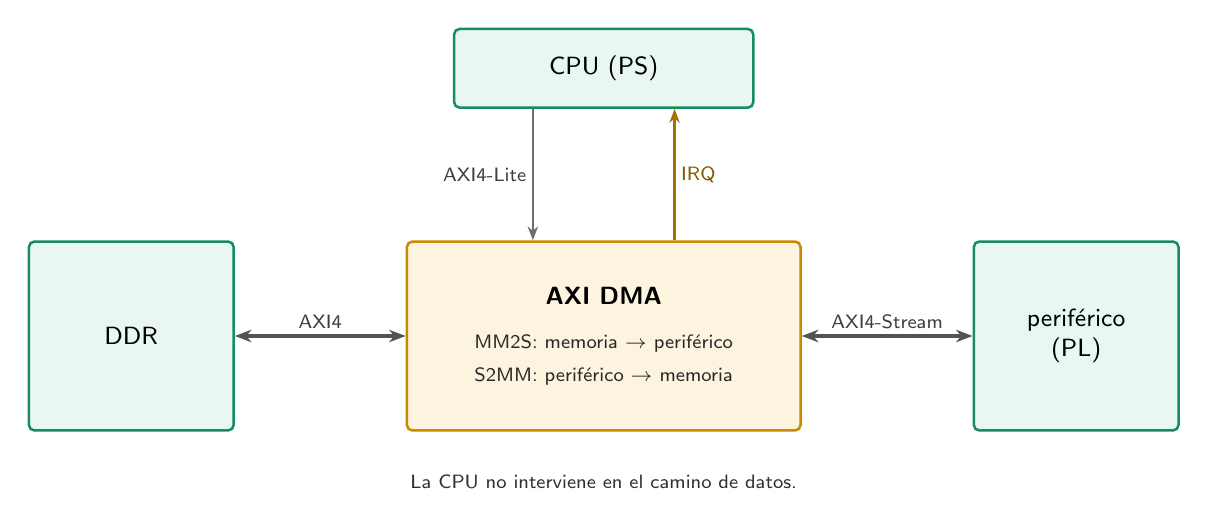
\begin{tikzpicture}[x=1cm, y=1cm]

% ===================== Fila del camino de datos =====================
\node[ext, minimum width=2.6cm, minimum height=2.4cm] (ddr) at (0,0) {DDR};
\node[ip,  minimum width=5.0cm, minimum height=2.4cm] (dma) at (6,0)
     {\textbf{AXI DMA}\\[5pt]
      \sub{MM2S: memoria $\rightarrow$ perif\'erico}\\[1pt]
      \sub{S2MM: perif\'erico $\rightarrow$ memoria}};
\node[ext, minimum width=2.6cm, minimum height=2.4cm] (pl) at (12,0)
     {perif\'erico\\(PL)};

% ===================== CPU, aparte =====================
\node[ext, minimum width=3.8cm, minimum height=1.0cm] (cpu) at (6,3.4) {CPU (PS)};

% ===================== Camino de datos =====================
\draw[data] (ddr.east) -- (dma.west) node[midway, above, rot] {AXI4};
\draw[data] (dma.east) -- (pl.west) node[midway, above, rot] {AXI4-Stream};

% ===================== Configuracion e interrupcion =====================
\draw[ctrl] ($(cpu.south)+(-0.9,0)$) -- ($(dma.north)+(-0.9,0)$)
      node[midway, left, rot] {AXI4-Lite};
\draw[irq]  ($(dma.north)+(0.9,0)$) -- ($(cpu.south)+(0.9,0)$)
      node[midway, right, rot, text=cIP!55!black] {IRQ};

% ===================== Idea clave =====================
\node[rot, text=cRef!35!black] at (6,-1.85)
     {La CPU no interviene en el camino de datos.};

\end{tikzpicture}
\end{document}
